\documentclass[12pt]{article}
\usepackage[a4paper, margin=2cm]{geometry}
\usepackage[english]{babel} % To obtain English text with the blindtext package
\usepackage{blindtext}
\usepackage{graphicx} % Required for inserting images
\usepackage{array, multirow} % For extra column formatting
\usepackage{amsmath, amssymb, cancel} %for equation environment
\usepackage{float}
\usepackage{parskip} % For gaps between para
\usepackage{setspace}
\usepackage{pdfpages}
\usepackage{abstract}
\usepackage[export]{adjustbox}
\usepackage{emptypage}
\usepackage{tocloft}
\usepackage[nottoc]{tocbibind}
\usepackage{hyperref, url}
\usepackage[table]{xcolor}
\usepackage{minted}
    \usemintedstyle{monokai}
\usepackage{caption,subcaption}
    \captionsetup{font=footnotesize,labelfont=bf}
\usepackage{tcolorbox}
    \newtcolorbox{mintedbox}{
        colback=backcolour,
        boxrule=0pt,
        sharp corners,
        width=\linewidth,
        left=0pt, right=0pt,
        top=3pt, bottom=3pt
    }
\usepackage{titlesec}

\pagenumbering{arabic}

\cftsetindents{section}{0em}{2em}
\cftsetindents{subsection}{0em}{2em}

\renewcommand\cfttoctitlefont{\hfill\Large\bfseries}
\renewcommand\cftaftertoctitle{\hfill\mbox{}}

\graphicspath{ {./images/} }

\definecolor{blurple}{HTML}{5865F2}
\definecolor{backcolour}{HTML}{272823}

\hypersetup{
    colorlinks=true,
    linkcolor=black,
    urlcolor=black,
    citecolor=blurple,
}

\urlstyle{same}

\renewcommand{\arraystretch}{1.3}

\setcounter{secnumdepth}{5}
\setcounter{tocdepth}{5}
\newcommand\simpleparagraph[1]{%
  \stepcounter{paragraph}\paragraph*{\theparagraph\quad{}#1}}

%%%%%%%%%%%%%%%%%%%%%%%%%%%%%%%%%%%


\title{PHYC20080 Exp.4 Interference}
\author{Joana Adao}
\date{\today}

\begin{document}

\begin{titlepage}
    \begin{center}

        \begin{figure}[ht]
            
\includegraphics[width=\textwidth]{UCDLogo.png}
        \end{figure}
        
        \begin{figure}
            \centerline{
\includegraphics[width=\paperwidth]{UCDBanner.png}}
        \end{figure}

        \vspace{4cm}

        {\LARGE \bfseries PHYC20080 Fields, Waves and Light}\\
        \vspace{0.75cm}
        {\Large Experiment No.4 Interference and Diffraction}
        
        \vspace{1cm}
    
    {\Large \textbf{25 March 2025}}
    
    \vspace{2cm}
    
    {\large \textbf{by Joana C.C. Adao (Student No. 23311051)}}\\
    \vspace{.25cm}
    {\large With Beau Etac}\\
    \vspace{0.25cm}
    {\large Tuesday 16.00-18.00 Slot}\\
    {\large Nicki (Coordinator)}

    \end{center}
    
   \clearpage

\end{titlepage}


\tableofcontents
\thispagestyle{empty}

\newpage

\begin{abstract}
\addtocontents{toc}{\protect\contentsline{section}{\textbf{Abstract}}{\hfill}{}}
\thispagestyle{empty}

This experiment aimed to explore the principles of wave interference and diffraction through the single slit and Young's double slit experiment. With the use of a coherent light source, both experiments were successful in demonstrating these properties
by calculating the slit width (a) for the single slit experiment and the slit separation (d) for the double slit experiment. The results of (a) for two renditions of the single slit experiment were found to be \textbf{8.131 $\mathbf{\times 10^{-5} \: \pm}$ 6.776 $\mathbf{\times 10^{-6}}$ m} and
\textbf{1.630 $\mathbf{\times 10^{-4} \: \pm}$ 2.717 $\mathbf{\times 10^{-5}}$ m}. This same experiment was applied to find the width of a human hair, with the result of \textbf{1.222 $\mathbf{\times 10^{-4} \: \pm}$ 1.528 $\mathbf{\times 10^{-5}}$ m}, which was within the range of typical human hair thickness of 
1.7$\times 10^{-5}$-1.80$\times 10^{-4}$ m. For the Young's double slit experiment the result of (d) was found to be \textbf{2.845 $\mathbf{\times 10^{-7} \: \pm}$ 3.230 $\mathbf{\times 10^{-8}}$ m}. These findings validated the wave nature of light and further reinforced key concepts in optics, exploring how
these properties can be applied in holography and crystalography.
 
\end{abstract}
\newpage

%%%%%%%%%%%%%%%%%%%%%%%%%%%%%%%%%%%

\setcounter{page}{1}
\section{Theory} \label{sec:1}

\subsection{Wave Nature of Light}

The wave nature of light was first demonstrated through slit experiments, in which light displayed diffraction (see §\ref{sec:1.2}) and interference (see §\ref{sec:1.3}) behaviours. Therefore, it was concluded that light
is a \textit{transverse, eletromagnetic wave}. The transverse wave nature of light can be demonstrated through polarisation of the wave \cite{natureoflight}.

\subsection{Diffraction} \label{sec:1.2}

Diffraction is the way light waves "bend" around barriers, such as a corner or through an opening, and consequently spread out. The diffraction patterns formed are parallel lines.
Diffraction is a specialised case of light scattering, such that when light encounters an object with regularly repeating openings (such as diffraction gratings) it produces an orderly diffraction pattern.
\cite{diffraction1}. 

\subsubsection{Fresnel Diffraction}

Fresnel diffraction is a near-field approximation of the Kirchoff or Rayleigh-Sommerfield diffraction integral, which describes how a wave propagates after encountering an obstacle. Fresnel's approximation
specifically pertains to when the recording screen is close in distance to the slits. Typically, this leads to more complex interference patterns (see Figure \ref{fig:2}) \cite{fresnelfraunhofer}.

\begin{figure}[H]
    \centering
    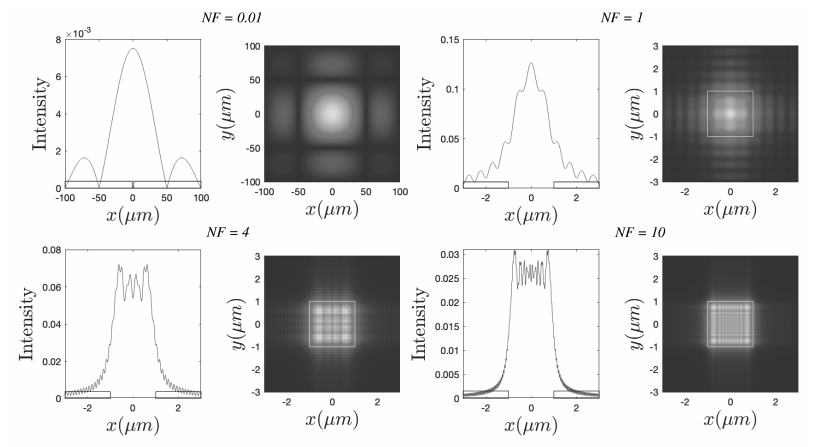
\includegraphics[width=.85\textwidth]{fresnel patterns.png}
    \caption{Example of intensities of Fresnel fields of a square opening, shown as contours and in cross-section for different distances, which increase from the lower right to the upper left.
    The upper left pattern is equal to the Fraunhofer pattern \protect\cite{fresnelfraunhofer}.}
    \label{fig:2}
\end{figure}

The minima condition for Fresnel diffraction is given as,

\vspace{-2ex}
\begin{gather*}
    \frac{x}{z} = (2m + 1) \frac{\lambda}{2a}
\end{gather*}

and maxima on,

\vspace{-2ex}
\begin{gather*}
    \frac{x}{z} = m \frac{\lambda}{a}
\end{gather*}

with $m$ as an integer of the order of the maxima/minima, $z$ as the distance between the screen and the opening (slit), $\lambda$ as the wavelength of light, $a$ as the half-width of the slit ($2a$ being the full width),
and $x$ as the distance of a point from the centre of the diffraction pattern on the screen \cite{fresnelfraunhofer}.

\subsubsection{Fraunhofer Diffraction}

Fraunhofer diffraction is a far-field approximation of the Kirchoff or Rayleigh-Sommerfield diffraction integral. Fraunhofer's approximation specifically pertains to when the recording screen is a considerable distance from the oopening (slit) \cite{fresnelfraunhofer}.
The resuting interference patterns are most associated with the traditional single slit (see §\ref{sec:1.4}) and double slit (see §\ref{sec:1.5}) experiments.

The intenisty pattern of a single-slit diffraction experiment is given by,

\vspace{-2ex}
\begin{gather*}
    I(\theta) = I_0 [sinc(\beta)]^2 \qquad , \qquad I(\theta) \propto \left( \frac{sin(\beta)}{\beta} \right)
\end{gather*}

where

\vspace{-2ex}
\begin{gather*}
    \beta \equiv \frac{ak sin \theta}{2} = \frac{a \pi sin \theta}{\lambda} \qquad , \qquad k = \frac{2 \pi}{\lambda}
\end{gather*}

where $I$ is the intensity, $a$ is the slit width, $k$ is the wavenumber, $\theta$ is the angle the fringe makes from the central axis, $\lambda$ is the wavelegnth \cite{fraunhofer}.

\subsection{Interference} \label{sec:1.3}

Interference, when in reference to light and optics, occurs when two or more light beams collide and are superimposed. Interference occurs when spatial and temporal phases overlap for both light beams,
the phase is \textit{coherent}, and the light has non-orthogonal polarisation states \cite{Paschotta_2005_interference}.

\subsubsection{Laser Properties for Interference} \label{sec:1.3.1}

Lasers are \textbf{highly monochromatic and coherent} which allows for stable interference patterns to be formed, making it much simpler to read and see the interference fringes.

\paragraph{Monochromaticity} \label{sec:1.3.1.1} \leavevmode\\
\vspace{-3ex}

For stable interference, the source itself must be stable such that the light is emitted at a single wavelength \cite{princelaser}.
Any variation in wavelength would cause the fringes to become "blurred". The laser being monochromatic ensures the fringes remain sharp and stable (well-defined).

\begin{figure}[H]
    \centering
    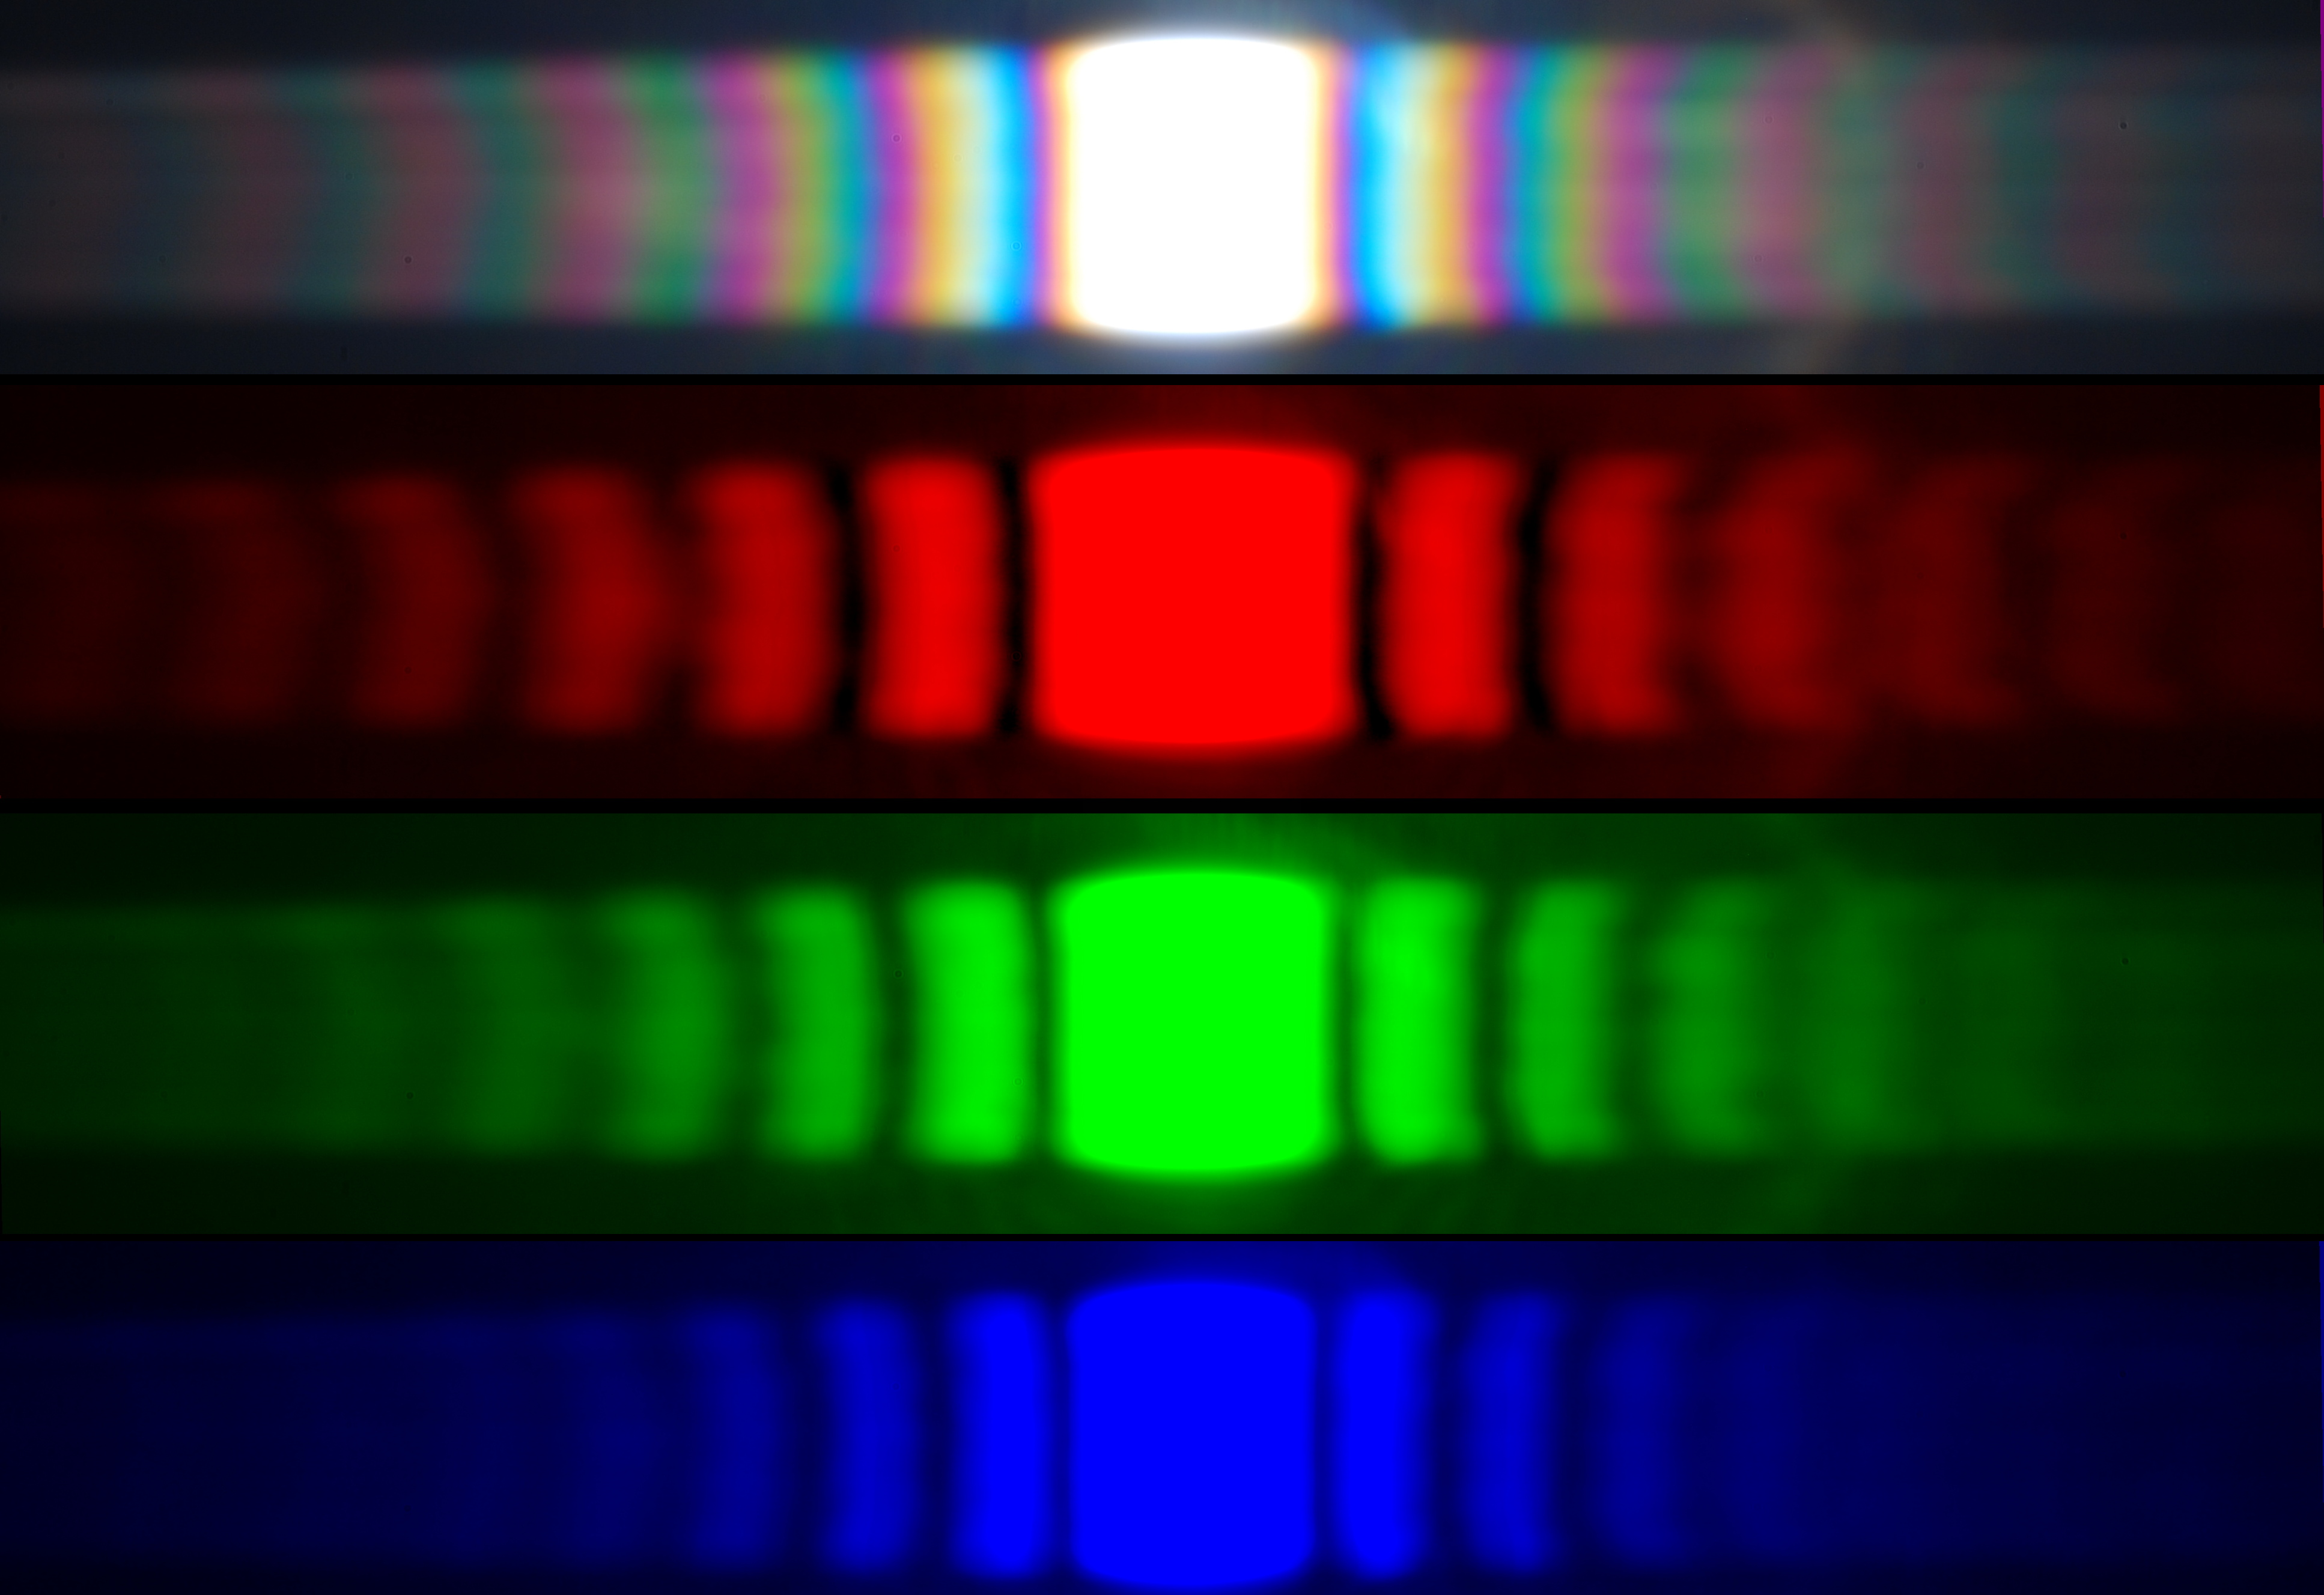
\includegraphics[width=.5\textwidth]{interference patterns.jpg}
    \caption{\centering Double slit experiment for different coloured lights (white, red, green, blue) \protect\cite{holoimg2}.}
    \label{fig:4}
\end{figure}

As can be seen in Figure \ref{fig:4}, the interference patterns from the monochromatic light sources (red, green, blue) appear much sharper than the "blurred" interference pattern of the white light (top)
due to the range of wavelengths present in white light. White light appears "blurry" due to the wavelength of each colour being diffracted at a alightly different angle.

\paragraph{Coherence} \label{sec:1.3.1.2} \leavevmode\\
\vspace{-3ex}

For there to be stable interference, the light source must have a fixed phase relationship at different points in time and/or space \cite{wolf2007introduction}.
This property ensures that light beams maintain a consistent phase difference, allowing them to interfere and create the fringes of greater and lesser amplitudes
\cite{Born_Wolf_Bhatia_Clemmow_Gabor_Stokes_Taylor_Wayman_Wilcock_1999}.

\begin{figure}[H]
    \centering
    \begin{subfigure}[b]{.45\textwidth}
        \centering
        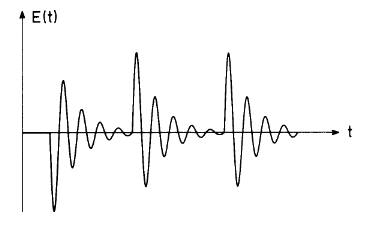
\includegraphics[width=\linewidth]{incoherent source.png}
        \caption{\centering Incoherent lamp light source}
        \label{fig:5a}
    \end{subfigure}
    \hspace{-.5em}
    \begin{subfigure}[b]{.45\textwidth}
        \centering
        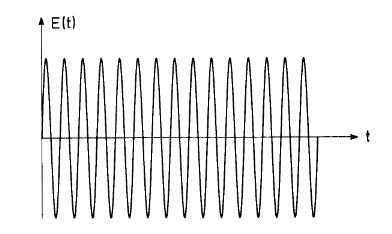
\includegraphics[width=\linewidth]{coherent source.png}
        \caption{\centering Coherent laser light source}
        \label{fig:5b}
    \end{subfigure}
    \caption{(a) The electric field strength E(t) of light of a lamp consists of uncorrelated individual wave tracks.
    (b) Laser light consists of a single coherent very strong wave track. \protect\cite{haken1986laser}.}
    \label{fig:5}
\end{figure}

A graphical representation of an incoherent (\ref{fig:5a}) and a coherent (\ref{fig:5b}) can be seen in Figure \ref{fig:5} above. Visually, it can be understood why a coherent
source is necessary for the production of stable interference fringe patterns.

\subsection{Single Slit Experiment} \label{sec:1.4}

For a single slit experiment the central maximum will be much larger than the adjacent and subsequent maxima, with the intensity decreasing rapidly from the centre. The interference patterns form
as the wave arrives either in or out of phase to a common location (the screen). The central maximum is so bright because majority of the light will arrive straight-on and therefore in phase \cite{urone2012collegesingle}.

The following equation describes the minima of the fringe pattern,

\vspace{-2ex} \label{eq:1}
\begin{gather}
    a sin \theta = m \lambda
\end{gather}

where $a$ is the slit width, $\theta$ is the angle, $m$ is an integer, and $\lambda$ is the wavelength. It can then be found that the slit width is (for $\theta$ small $\approx sin \theta$) \cite{UCDinterference}:

\vspace{-2ex}
\begin{gather} \label{eq:2}
    a = \lambda \: \frac{D}{Y}
\end{gather}

with $D$ as the distance from the pattern to the slit, and $Y$ as the distance from the central maximum to the first minimum.

\subsection{Double Slit (Young's) Experiment} \label{sec:1.5}

Thomas Young was the first to prove that light was indeed also a wave by means of the double slit experiment (see Figure \ref{fig:1}). Light must interact somthing small, such as the small opening of the slits, in order to
exhibit wave-like behaviour and the light must also be coherent \cite{urone2012collegedouble}.

\begin{figure}[H]
    \centering
    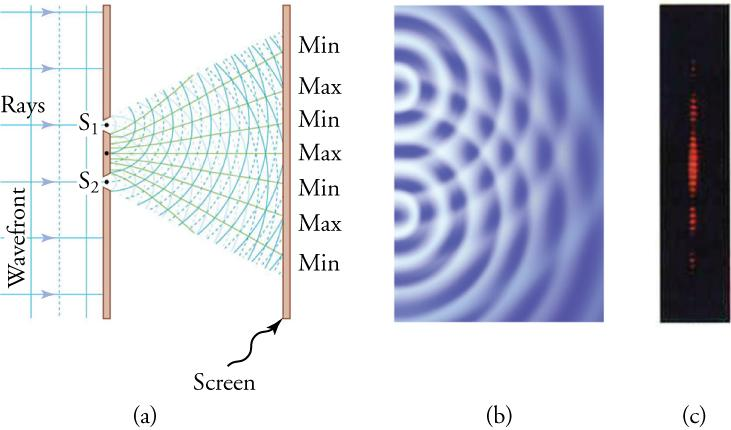
\includegraphics[width=.7\textwidth]{diffraction pattern.jpg}
    \caption{ Double slits produce two sources that interfere. (a) Diffraction of light as it encounters a barrier, forming dark and bright regions of destructive and constructive interference, respectively.
    (b) Double-slit interference pattern for diffracted light. (c) Pattern seen when light falls onto a screen. \protect\cite{urone2012collegedouble}}
    \label{fig:1}
\end{figure}

The equation for the double slit experiment imply there are a series of dark and bright fringes formed due to destructive and constructive interference of the light. The cloesr the slits are to each other, the more spread out the fringes will be (see Figure \ref{fig:3}).
This can be observed by examining the equation \cite{urone2012collegedouble},

\vspace{-2ex}
\begin{gather} \label{eq:3}
    d sin \theta = n \lambda
\end{gather}

where $n$ is an integer, $\theta$ is the angle, $\lambda$ is the wavelength, and $d$ is the distance between the slits.

\begin{figure}[H]
    \centering
    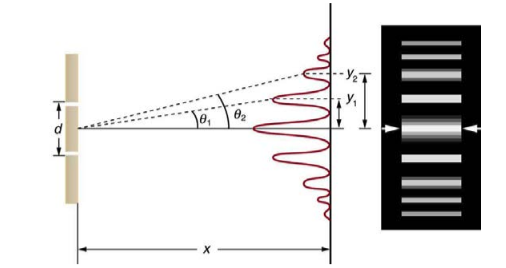
\includegraphics[width=.7\textwidth]{youngs slit.png}
    \caption{\centering The interference pattern for a double slit \protect\cite{urone2012collegedouble}.}
    \label{fig:3}
\end{figure}

When the angle is small, the approximation $sin \theta \approx \theta$ may be used to get

\vspace{-2ex}
\begin{gather}
    n \lambda \approx d \theta
\end{gather}

therefore the angular separation between adjacent maxima is

\vspace{-2ex}
\begin{gather} \label{eq:5}
    \frac{\lambda}{d} = \frac{y}{D}
\end{gather}

where $y$ is the linear separation between adjacent maxima, and $D$ is the distance from the pattern to the slit \cite{UCDinterference}.

\subsection{Applications of Interference and Diffraction}

\textbf{Holography} is based on \textit{interference}. Holograms are formed when two mutually coherent light monochromatic laser sources, an object-illumating beam and reference beam, are superimposed onto a recording medium to form an interfence pattern. By recording both the phase
and amplitude of a wave, the wavefront, a 3D image reconstruction of the original object can be achieved when the hologram is illuminated by the reference beam \cite{Paschotta_2019_holography,ownholo}.

\textbf{Crystalography} is based on \textit{diffraction}. Particularly, Bragg diffraction forms the fundamental principles of this practice, in which x-rays bounce off the atoms in a crystal lattice planes (see Figure \ref{fig:6}). At certain angles, 
constructive interference patterns are formed. By measuring these angles and intensities, crystallographers can apply it to Bragg's Law, a version of Eq. \ref{eq:3}: $2d sin \theta = n \lambda$. This allows the crystallographers to find d, the interplanar spacing \cite{hansen2015diffraction}.

\begin{figure}[H]
    \centering
    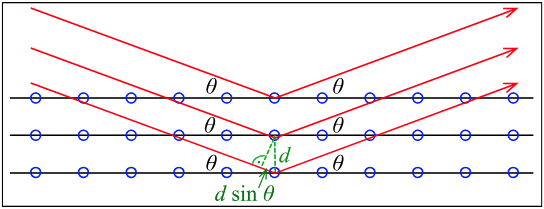
\includegraphics[width=.8\textwidth]{bragg lattice.png}
    \caption{Bragg diffraction as a specular reflection on semi-transparetn mirrors of lattice planes: constructive interference only for certain path differences \protect\cite{hansen2015diffraction}.}
    \label{fig:6}
\end{figure}

\section{Methodology} \label{sec:2}

Both parts of the experiment have the same setup (see Figure \ref{fig:7}). A laser light is used for its monochromatic and coherent properties (discussed in §\ref{sec:1.3.1}).

\begin{figure}[H]
    \centering
    \begin{subfigure}[H]{.55\textwidth}
        \centering
        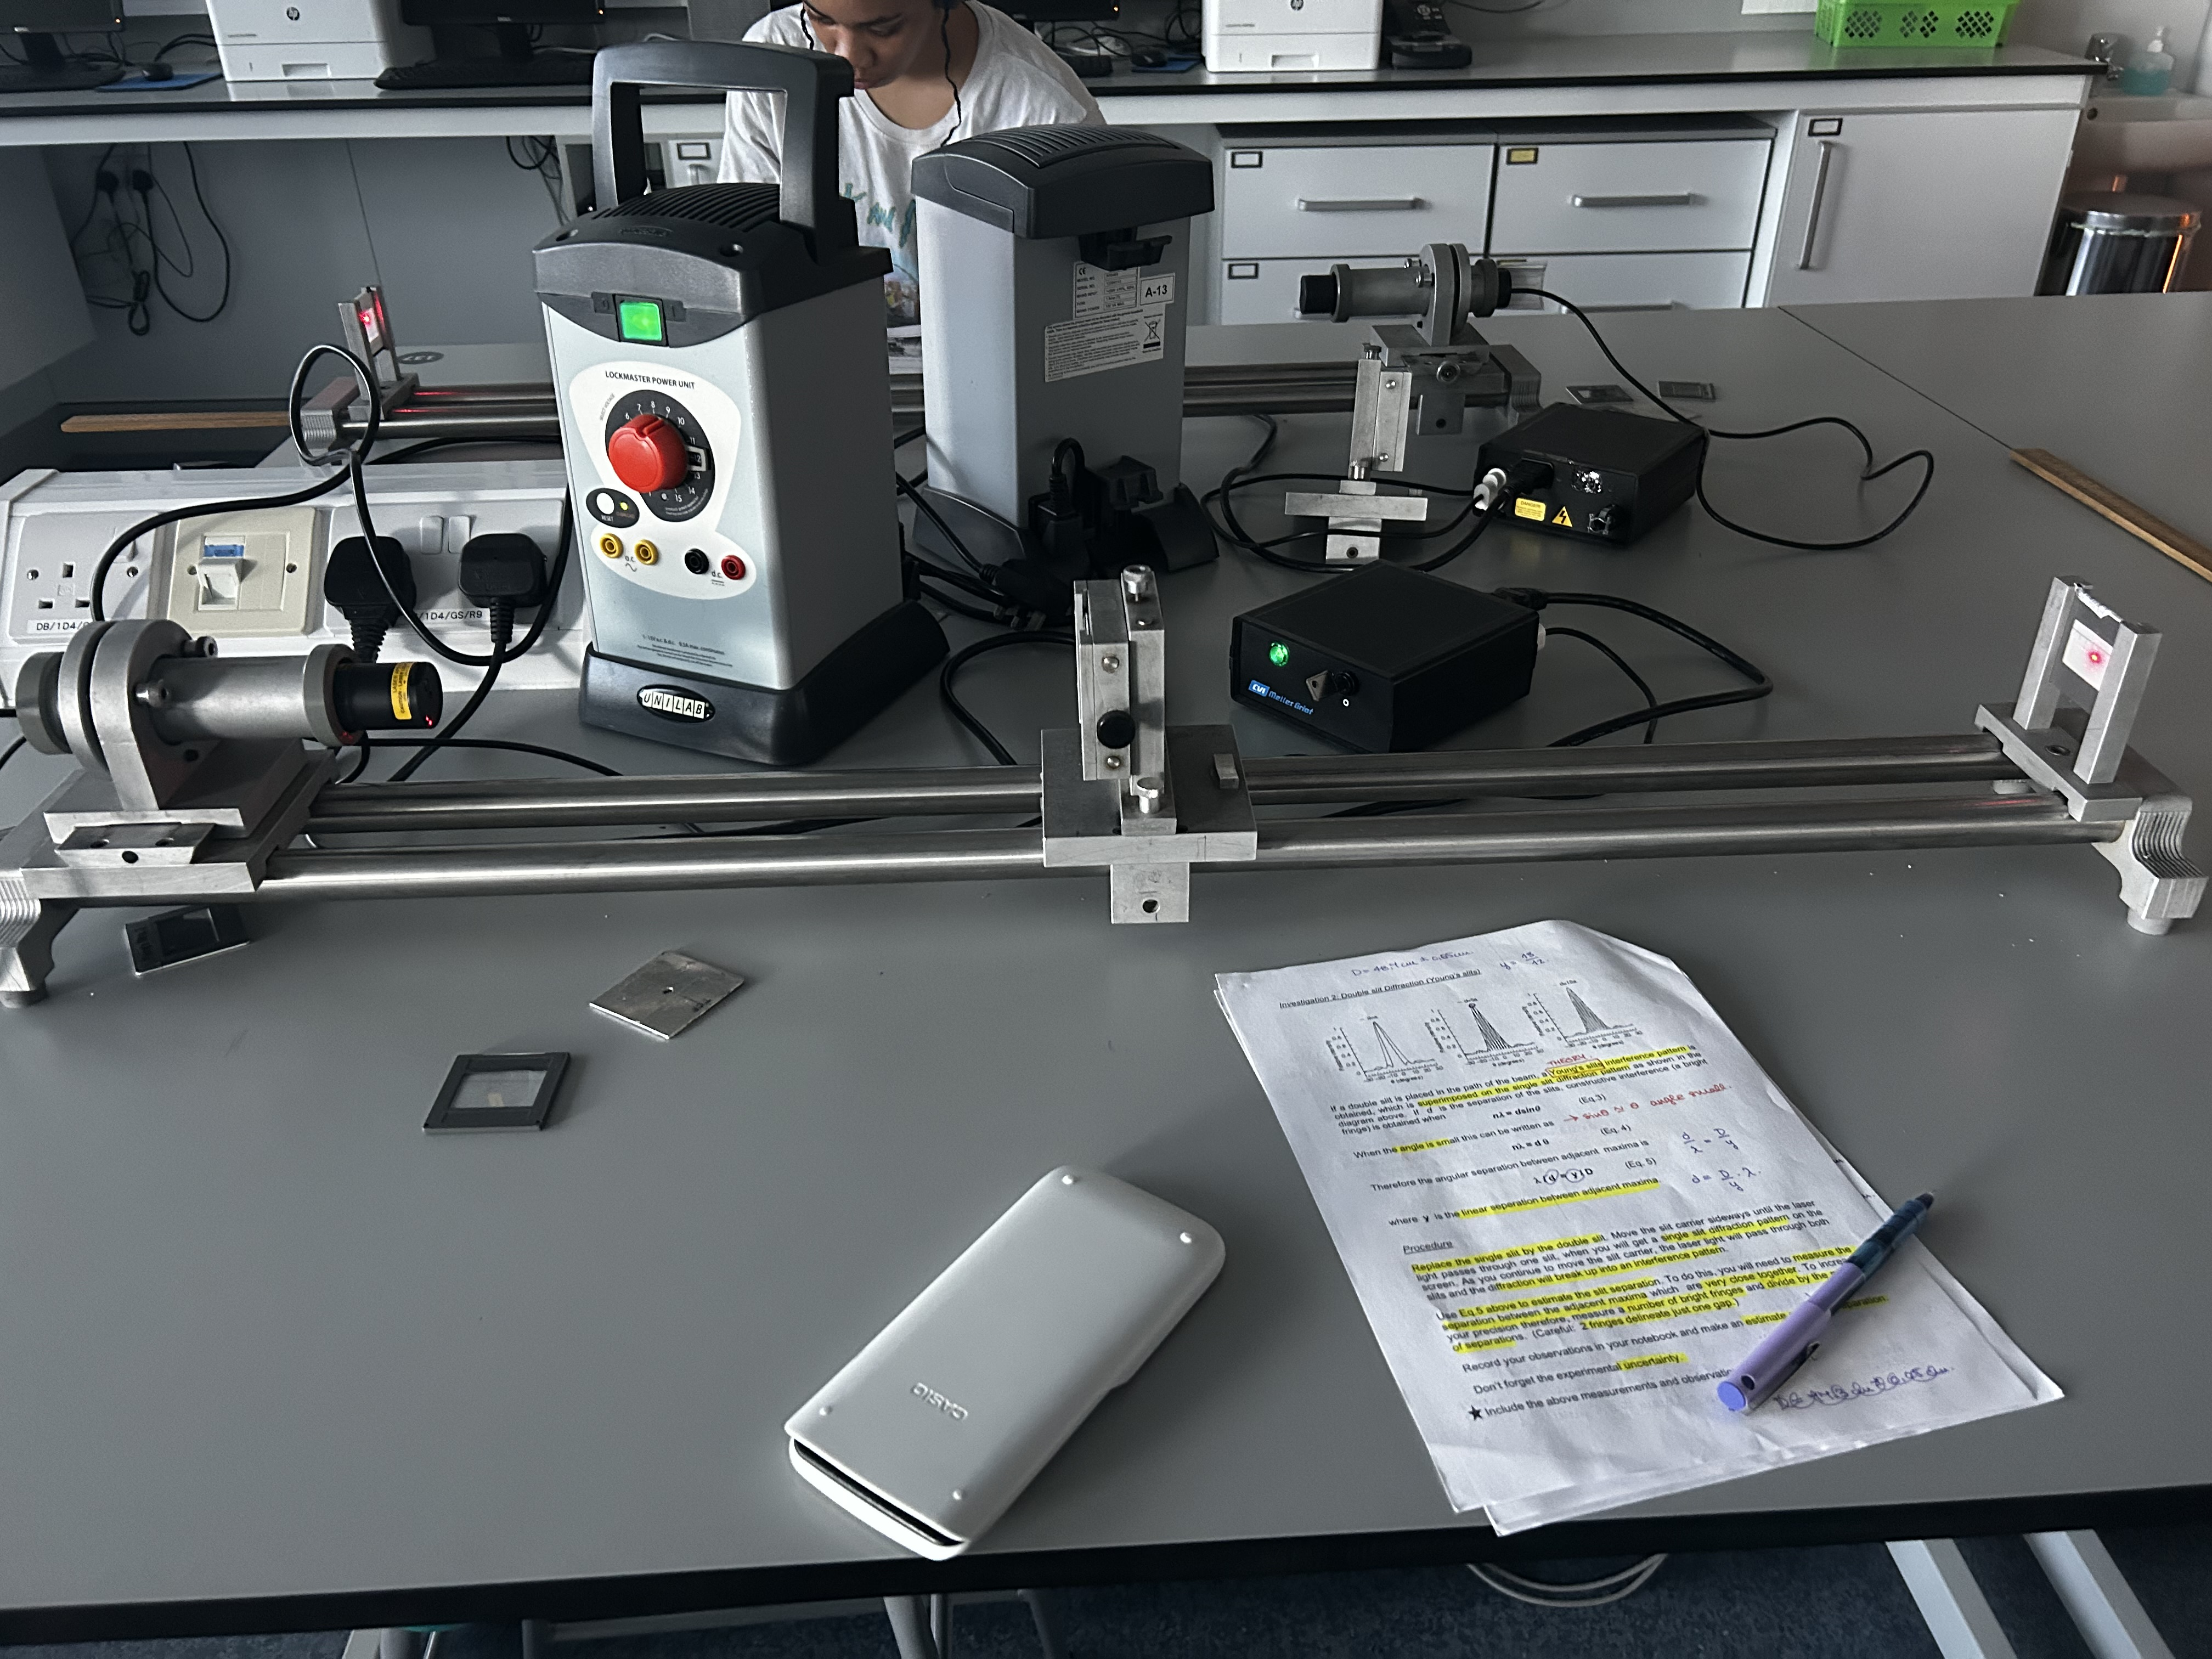
\includegraphics[width=\linewidth]{slits.jpeg}
    \end{subfigure}
    \hspace{-.5em}
    \begin{subfigure}[H]{.418\textwidth}
        \centering
        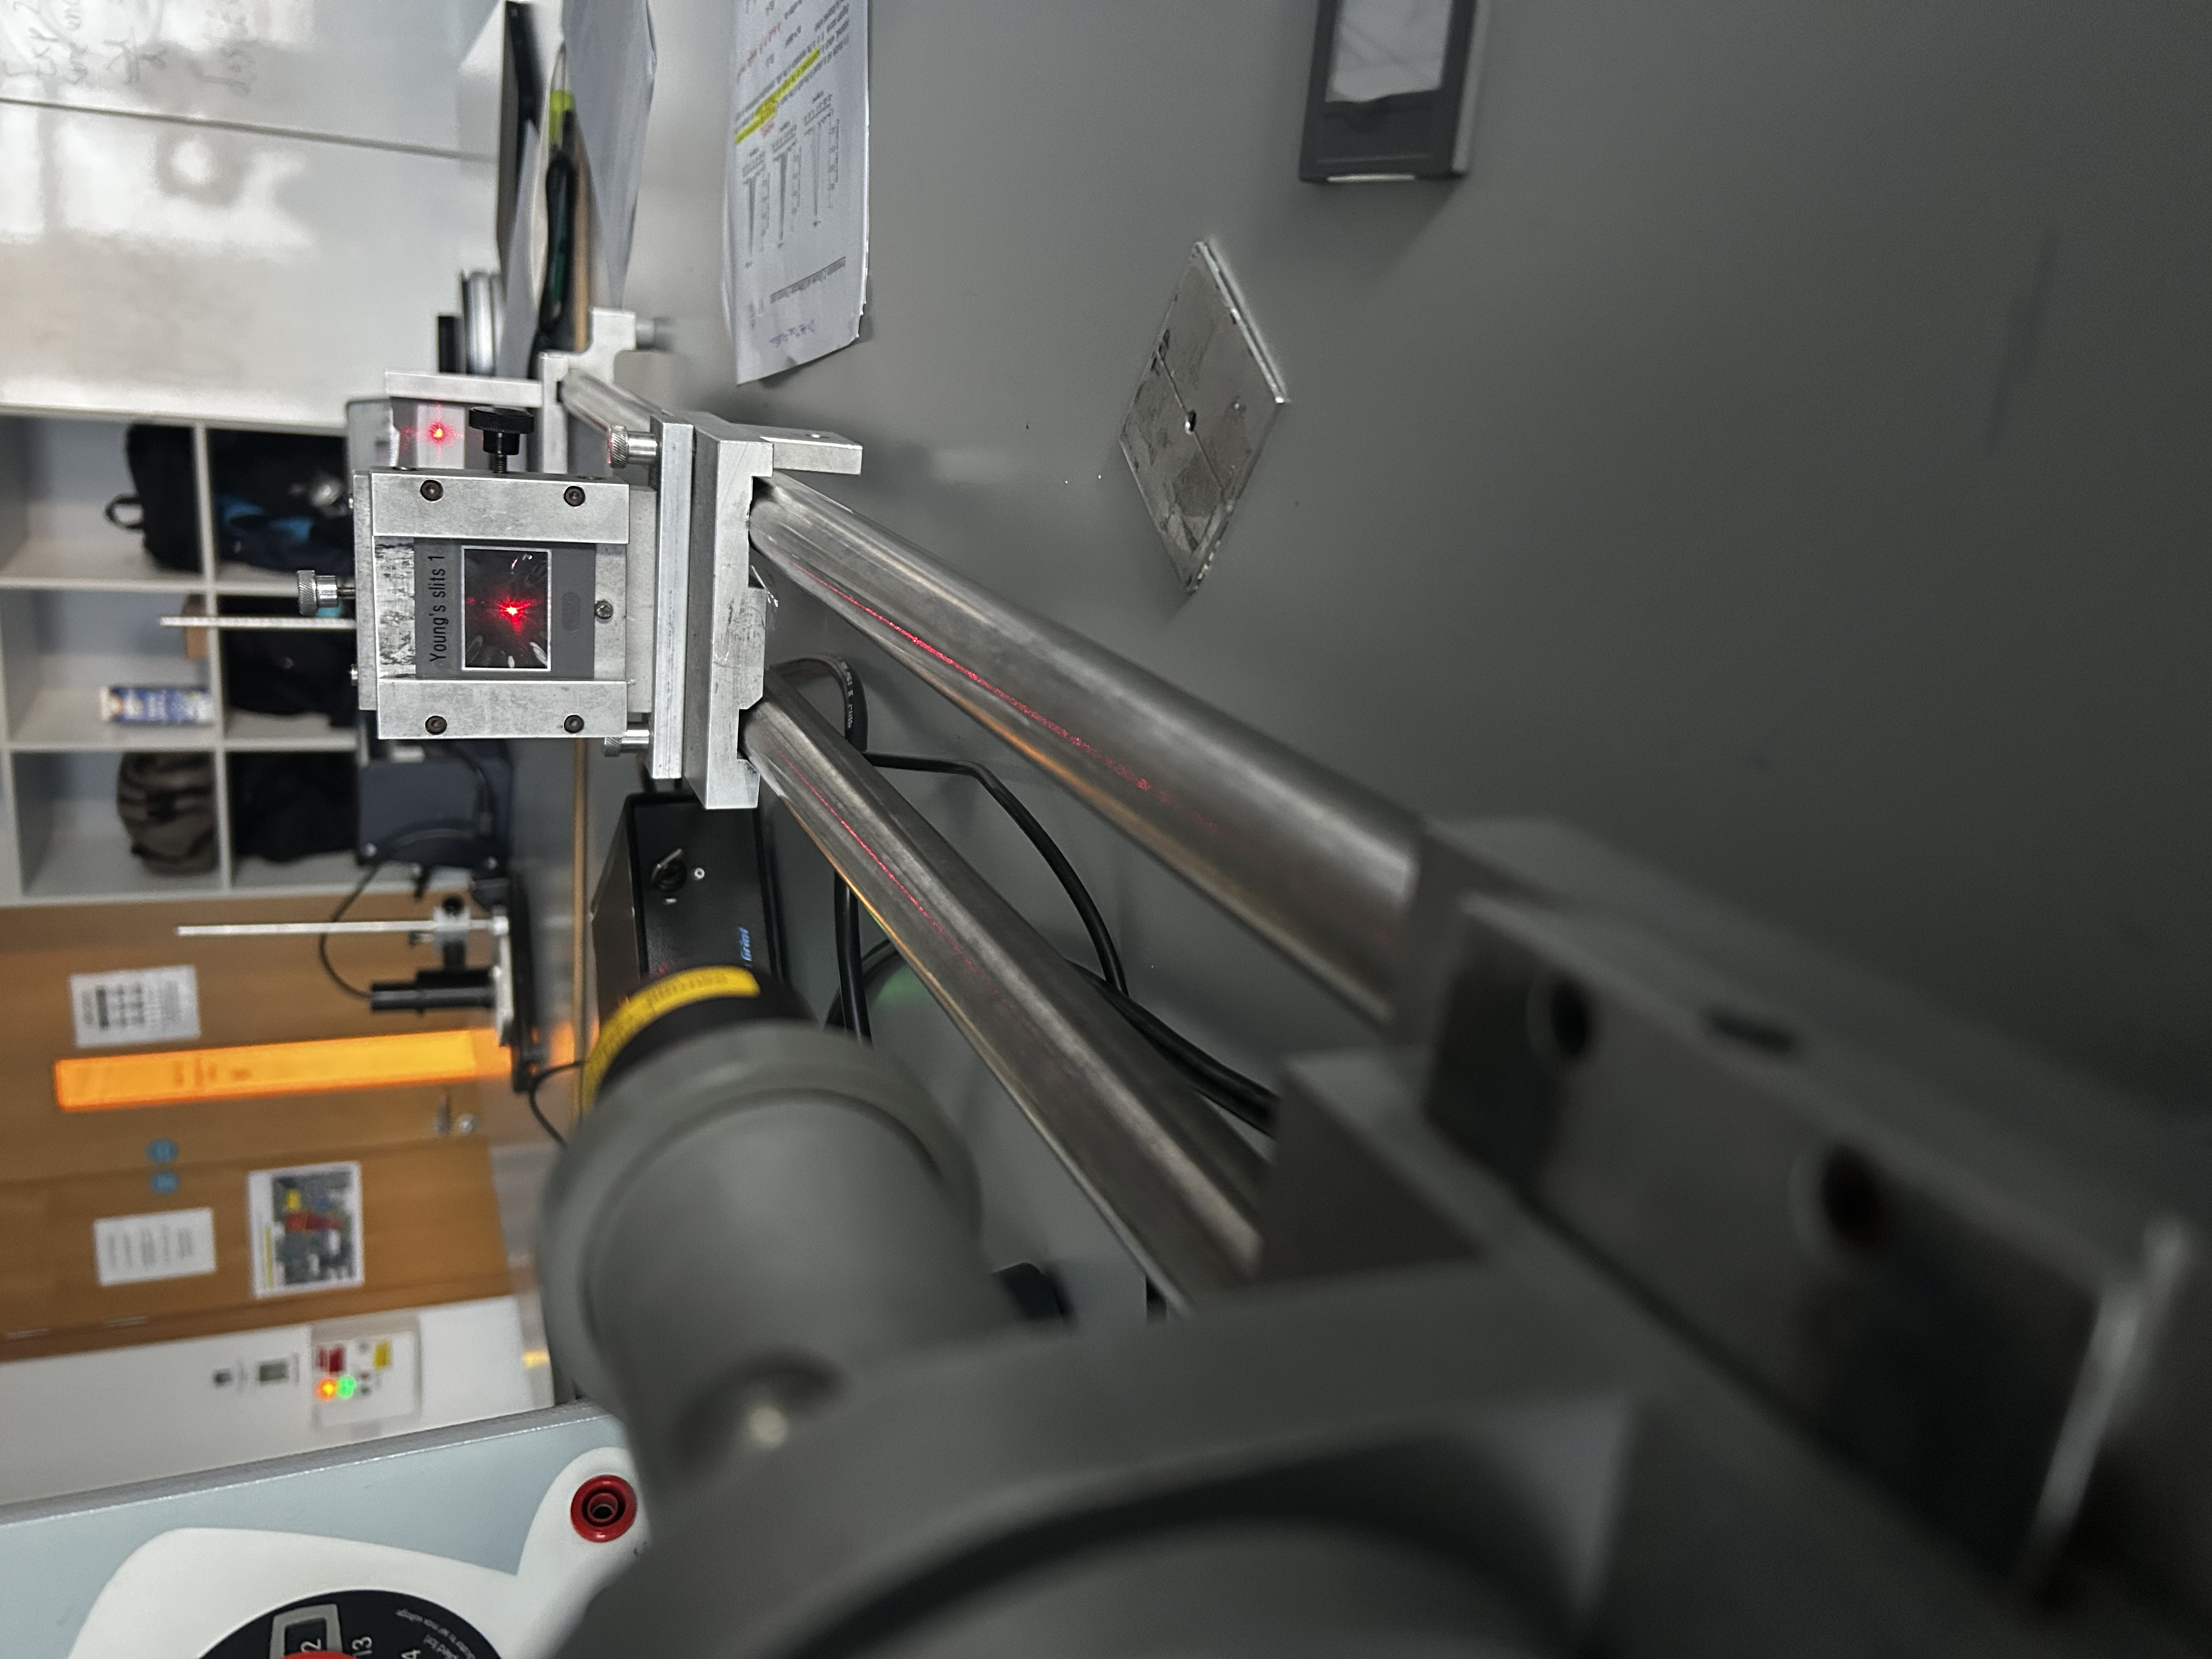
\includegraphics[width=\linewidth,angle=270]{candid laser shot.jpeg}
    \end{subfigure}
    \caption{Experimental setup, bridge (left) and laser position (right).}
    \label{fig:7}
\end{figure}

\subsection{Single Slit Experiment Method} \label{sec:2.1}

To reproduce the single slit experiment, a diffraction grating of a single slit must be used in the centre holder of the bridge. The laser light must be positioned
such that it passes through the slit and is seen on viewing screen (see Figure \ref{fig:7}). The distance D between the slit and the viewing screen should be as large as possible. This will make the interfence patterns appear larger (bigger angle) and thus the
distance between the minima adjacent to the central maximum will be easier to read and measure. The distance between the first order minima (see Figure \ref{fig:8}) will be 2Y.

\begin{figure}[H]
    \centering
    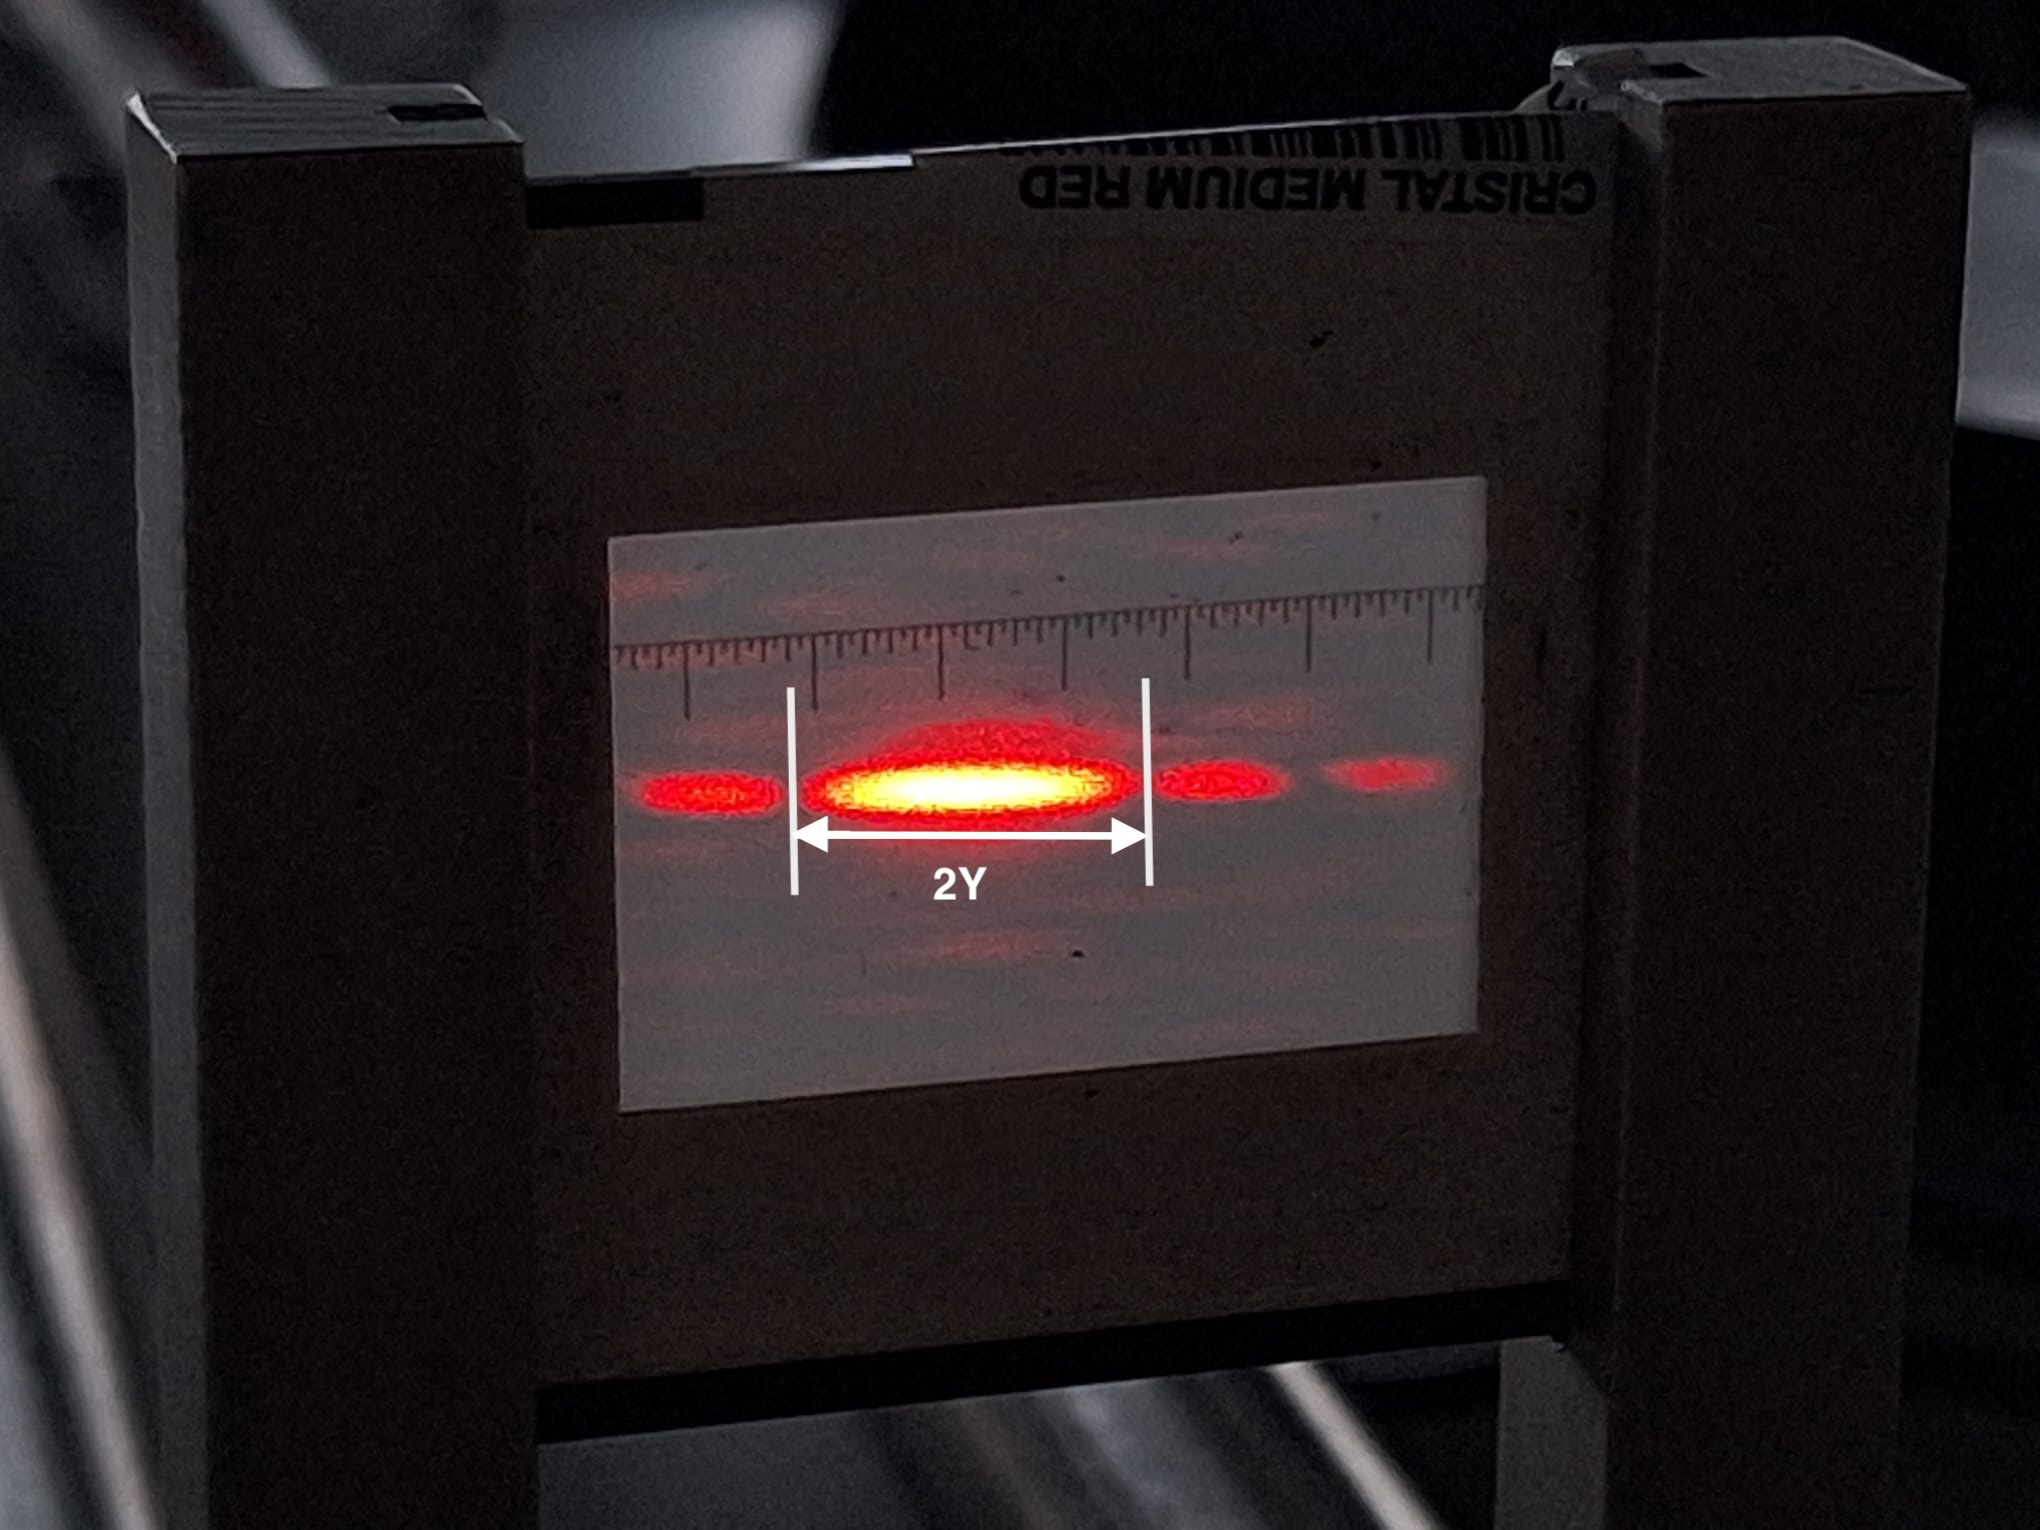
\includegraphics[width=.6\textwidth]{single slit diffraction.jpeg}
    \caption{Diffraction pattern as per the single slit experiment, with the distance between the first order minima 2Y labelled.}
    \label{fig:8}
\end{figure}

Using Eq. \ref{eq:2}, the width of the single slit (a) can be found as the wavelegnth of the laser light is given.

\subsection{Double Slit (Young's) Experiment Method} \label{sec:2.2}

To reproduce Young's slit experiment, a diffraction grating of a double slit must be used in the centre holder of the bridge. The laser light beam must be positioneed in such a way that it passes through both slits. Increasing the distance between the laser and the slits
will allow for this, but ensuring the largest distance possible between the viewing screen and the slits is still important to increases visibility of the minima. In the case of the double slit experiment,
two fringes account for a single gap (see Figure \ref{fig:9}).

\begin{figure}[H]
    \centering
    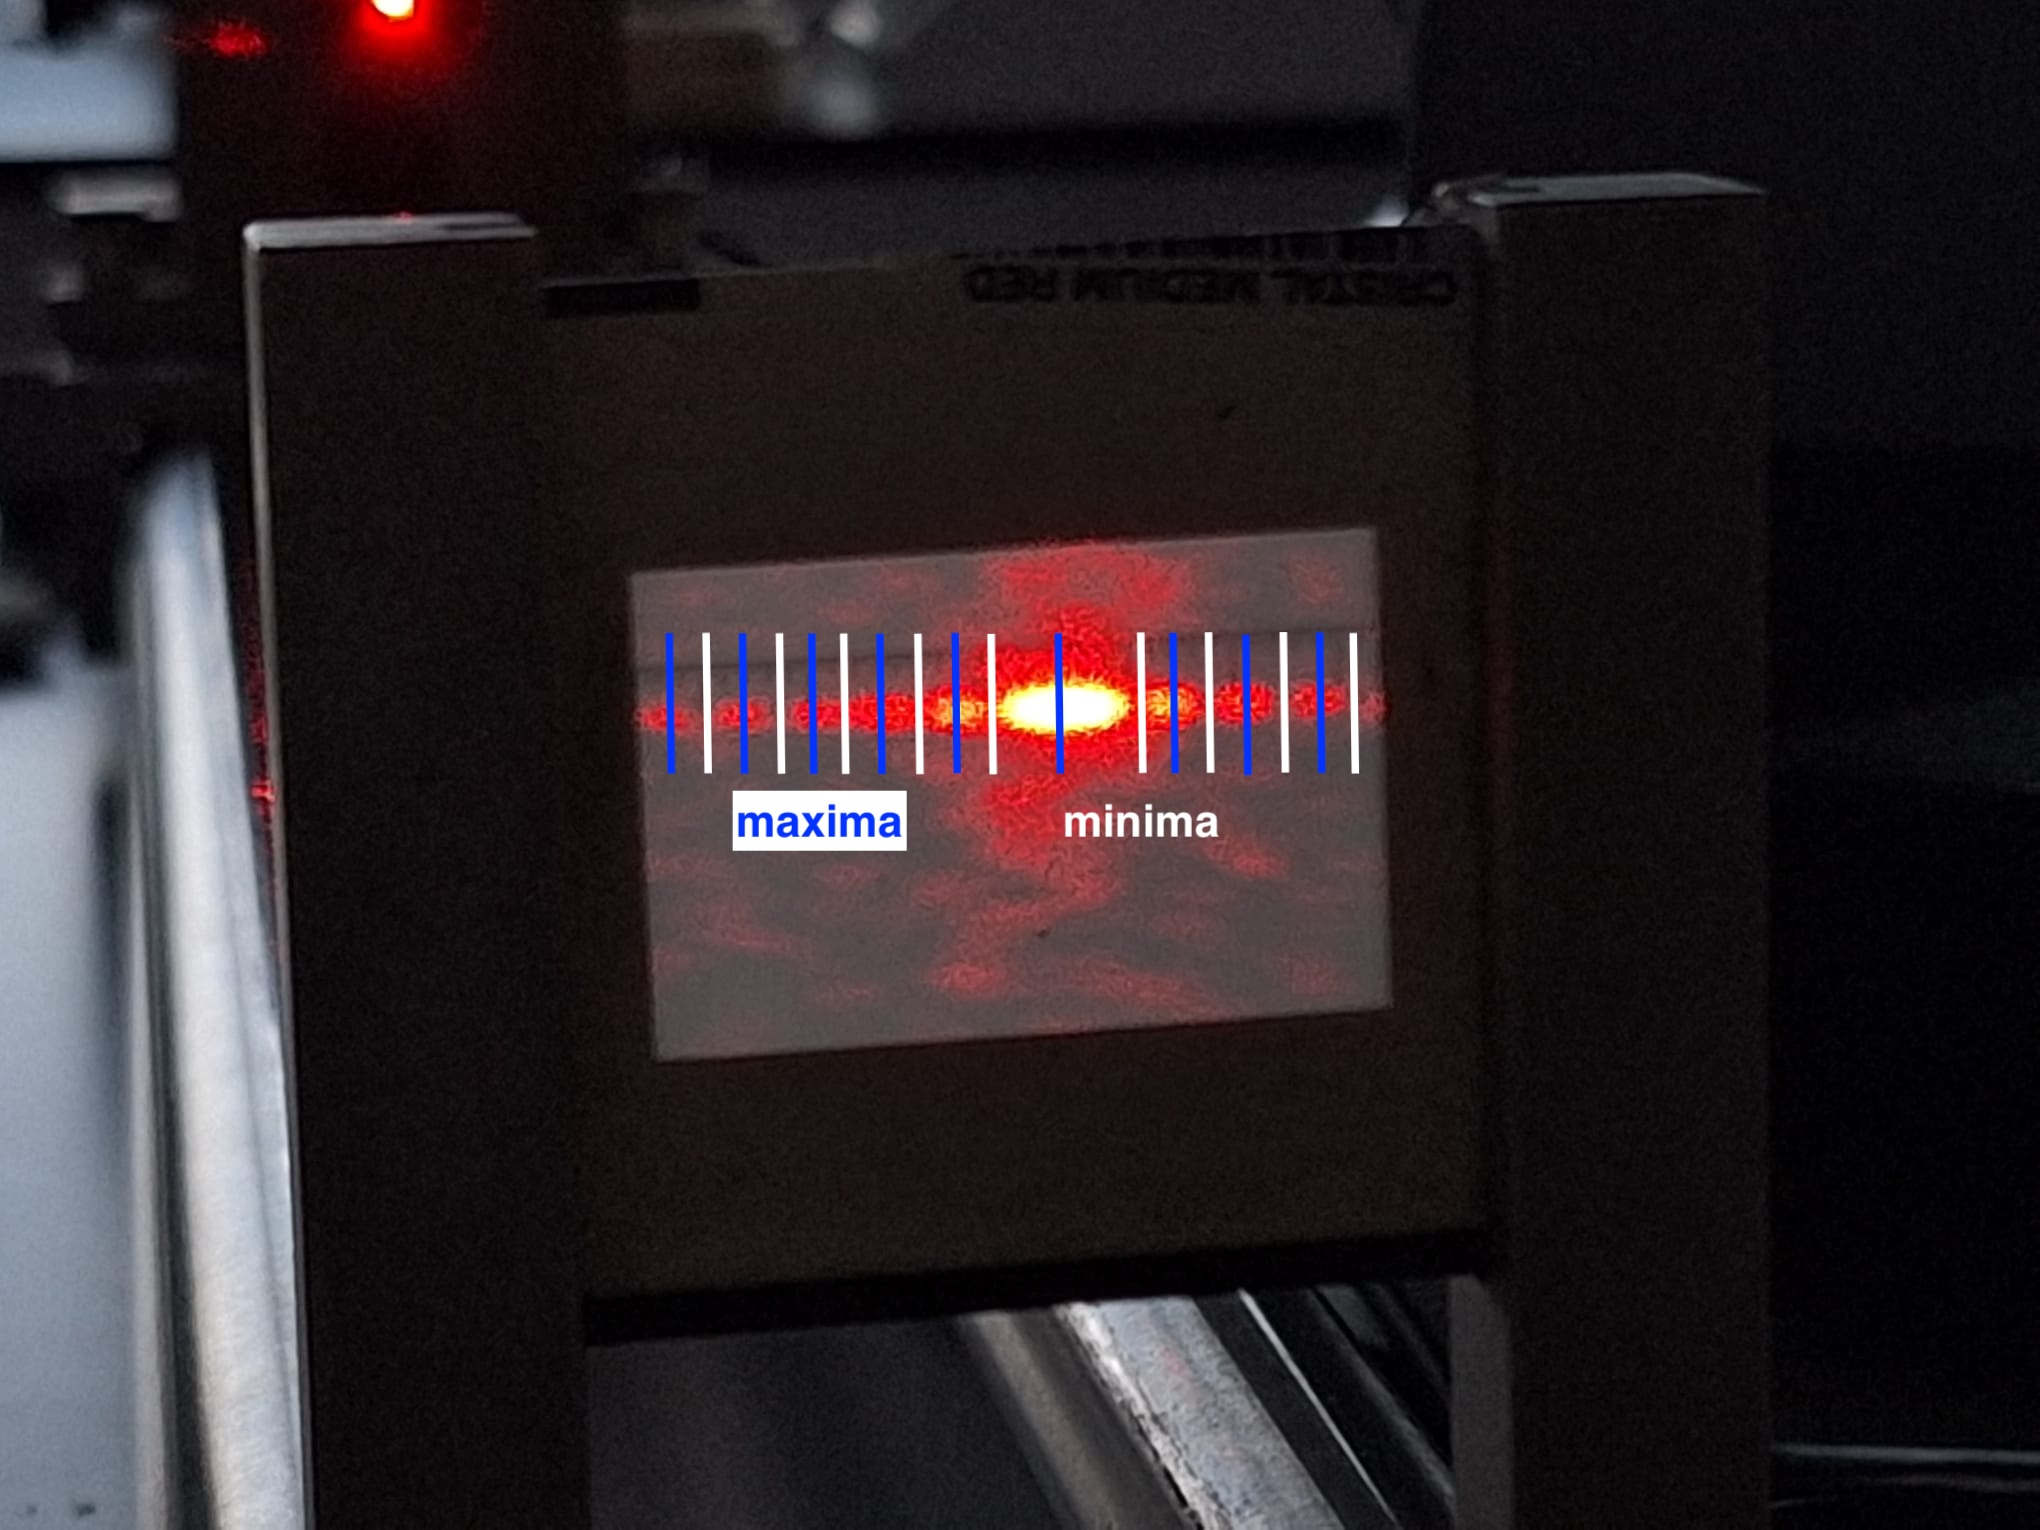
\includegraphics[width=.6\textwidth]{young diffraction.jpeg}
    \caption{Diffraction as per the double (Young's) slit experiment, with maxima (dark blue) and minima (white) labelled.}
    \label{fig:9}
\end{figure}

Using Eq. \ref{eq:5}, the slit separation (d) can be found, knowing that the linear separation between adjacent maxima y is the maxima divided by the minima.

\section{Results and Discussion} \label{sec:3}

\subsection{Single Slit Experiment Results}

The wavelength for the laser source was given as \textbf{632.8 nm}. With this, Eq. \ref{eq:2} can be used to find the slit width (a) for two renditions of the single slit experiment (Table \ref{tab:1}).

\begin{table}[H]
    \caption{Table of results for 2 single slits.}
    \label{tab:1}
    \resizebox{\textwidth}{!}{%
        \begin{tabular}{
        >{\columncolor[HTML]{EFEFEF}}c ccccc}
        \textbf{\#} &
        \textbf{\begin{tabular}[c]{@{}c@{}}D (m) \\ $\mathbf{\times 10^{-2}}$\end{tabular}} &
        \textbf{\begin{tabular}[c]{@{}c@{}}2Y (m)\\ (1st min.) $\mathbf{\times 10^{-3}}$\end{tabular}} &
        \textbf{\begin{tabular}[c]{@{}c@{}}$\mathbf{a = \lambda \: \frac{D}{Y}}$ (m)\\ (1st min.)\end{tabular}} &
        \textbf{\begin{tabular}[c]{@{}c@{}}2Y (m)\\ (2nd min.) $\mathbf{\times 10^{-3}}$\end{tabular}} &
        \textbf{\begin{tabular}[c]{@{}c@{}}$\mathbf{a = 2 \lambda \: \frac{D}{Y}}$ (m)\\ (2nd min.)\end{tabular}} \\ \hline
        \textbf{1} &
        77.1 $\pm$ 0.05 &
        12 $\pm$ 0.5 &
        8.131 $\times 10^{-5}$ $\pm$ 6.776 $\times 10^{-6}$ &
        24 $\pm$ 0.5 &
        4.066 $\times 10^{-5}$ $\pm$ 3.388 $\times 10^{-6}$ \\
        \textbf{2} &
        77.3 $\pm$ 0.05 &
        6 $\pm$ 0.5 &
        1.630 $\times 10^{-4}$ $\pm$ 2.717 $\times 10^{-5}$ &
        14 $\pm$ 0.5 &
        6.988 $\times 10^{-5}$ $\pm$ 4.992 $\times 10^{-6}$
        \end{tabular}%
    }
\end{table}

The results, as per Eq. \ref{eq:2}, for the second order minima for slit witdth a can be seen on the far right of Table \ref{tab:1}, but recall at second minima m = 2. If the results obtained for the slit width (a) at the second minima
were multiplied by 2 (m), the same answers as was achieved for the first minima would be obtained. This shows the relationship between the fringes and the slit width, which in turn showcases the relationship between the slit width and angle.

The same experiment can be recreated using human hair as the "slit", a similar barrier formed. The measurements for this rendition of the experiment were recorded in Table \ref{tab:2}.

\begin{table}[H]
    \caption{Table of results with human hair as a slit.}
    \label{tab:2}
    \resizebox{\textwidth}{!}{%
        \begin{tabular}{ccccc}
        \textbf{\begin{tabular}[c]{@{}c@{}}D (m) \\ $\mathbf{\times 10^{-2}}$\end{tabular}} &
        \textbf{\begin{tabular}[c]{@{}c@{}}2Y (m)\\ (1st min.) $\mathbf{\times 10^{-3}}$\end{tabular}} &
        \textbf{\begin{tabular}[c]{@{}c@{}}$\mathbf{a = \lambda \: \frac{D}{Y}}$ (m)\\ (1st min.)\end{tabular}} &
        \textbf{\begin{tabular}[c]{@{}c@{}}2Y (m)\\ (2nd min.) $\mathbf{\times 10^{-3}}$\end{tabular}} &
        \textbf{\begin{tabular}[c]{@{}c@{}}$\mathbf{a = \lambda \: \frac{D}{Y}}$ (m)\\ (2nd min.)\end{tabular}} \\ \hline
        77.3 $\pm$ 0.05 &
        8 $\pm$ 0.5 &
        1.222 $\times 10^{-4}$ $\pm$ 1.528 $\times 10^{-5}$ &
        16 $\pm$ 0.5 &
        6.114 $\times 10^{-5}$ $\pm$ 3.821 $\times 10^{-6}$
        \end{tabular}%
    }
\end{table}

The average hair width range is between 17-180 $\mu$m, or 1.7$\times 10^{-5}$-1.80$\times 10^{-4}$ m \cite{hairwidth}. The value calcualted above for the widht of the hair falls within this range, therefore the results
agree, proving the validity of this method in measuring the width of the hair.

The uncertainties for the slit width (a) is given by:

\vspace{-2ex}
\begin{gather*}
    \Delta a = a \sqrt{\left( \frac{\Delta D}{D} \right)^2 + \left( \frac{\Delta Y}{Y}^2 \right)^2}
\end{gather*}

\subsection{Double Slit (Young's) Experiment Results}

The laser remained the same at \textbf{632.8 nm}, hence \ref{eq:5} can be used to find the slit separation (d) for Young's double slit experiment, given in Table \ref{tab:3}.

\begin{table}[H]
    \centering
    \caption{Table of results for the double slit experiment.}
    \label{tab:3}
    \begin{tabular}{ccc}
    \textbf{D (m)}                                    & \textbf{y}                 & \textbf{$\mathbf{d = \lambda \: \frac{D}{y}}$ (m)}      \\ \hline
    48.7 $\times 10^{-2}$ $\pm$ 0.05 $\times 10^{-2}$ & $\frac{6.5}{6}$ $\pm$ 0.123 & 2.845 $\times 10^{-7}$ $\pm$ 3.230 $\times 10^{-8}$
    \end{tabular}%
\end{table}

The difference between the wavelegnth and the slit separation is found to be almost 1/2 (0.45). This small difference in value likely lead to distorted diffraction and interference patterns that appeared blurred,
making it harder to correctly read and differentiate between maxima and minima. 

The uncertainty for slit separation (d) is given by:

\begin{gather*}
    \Delta d = d \sqrt{\left( \frac{\Delta D}{D} \right)^2 + \left( \frac{\Delta y}{y}^2 \right)^2}
\end{gather*}

\vspace{2cm}

\section{Conclusion} \label{sec:4}

The single slit and Young's double slit experiments were both successful in results for validating the key concepts and properties of light discussed and explored in this report.

For the single slit experiment, the results \textbf{8.131 $\mathbf{\times 10^{-5} \: \pm}$ 6.776 $\mathbf{\times 10^{-6}}$ m} and \textbf{1.630 $\mathbf{\times 10^{-4} \: \pm}$ 2.717 $\mathbf{\times 10^{-5}}$ m} were calcualted for two different slit widths.
These results were found to agree with the same process done for the second minima, \textbf{4.066 $\mathbf{\times 10^{-5} \: \pm}$ 3.388 $\mathbf{\times 10^{-6}}$ m} and \textbf{6.988 $\mathbf{\times 10^{-5} \: \pm}$ 4.992 $\mathbf{\times 10^{-6}}$ m} respectively, which were found to be 
roughly half the values calculated for the first minima. This aligns with theoretical assumptions as m = 2 (Eq. \ref{eq:1}) for the second minima, indicating double the original wavelength.
Values also agreed with the theoretical ones when this experiment was conducted with use of a human hair, whose width was found to be \textbf{1.222 $\mathbf{\times 10^{-4} \: \pm}$ 1.528 $\mathbf{\times 10^{-5}}$ m}. The range of typical human hair is found to be 1.7$\times 10^{-5}$-1.80$\times 10^{-4}$ m \cite{hairwidth},
and the obtained value falls within this range.

For the Young's double slit experiment the slit separation was calculated to be \textbf{2.845 $\mathbf{\times 10^{-7} \: \pm}$ 3.230 $\mathbf{\times 10^{-8}}$ m}. The slit separation was found to be 0.45 of the wavelength of the laser source, which likely lead to distortions of the fringe pattern and presumed blurriness, 
meaning it was likely more difficult to read the maxima and minima of the pattern as the slit acted more as a single slit.

For future renditions of the single slit experiment, the distance between the viewing screen and the slit could be increased further to ensure clear and accurate readings of the fringe pattern. This could also be applied as an improvement for future renditions of the double slit experiment,
as greater distance between the screen and the slit would likely result in more fringes of the double slit diffraction. If there are more slits, however, it might turn difficult to count how many there are as they get closer together. If different colour laser light, like green for example, was used for this experiment,
results could be more diverse. A disadvantage of using a laser light with shorter wavelength would be smaller fringes that are closer together, but with better sharpness and clarity. Despite this, better analysis could be achieved by comparing numerical results between laser lights of different colours, mainting the slit width/separation
constant.

\newpage

%%%%%%%%%%%%%%%%%%%%%%%%%%%%%%%%%%%

\bibliographystyle{IEEEtran}
\bibliography{References} \label{sec:ref}

\vspace{1.5cm}

\listoffigures

\listoftables

\end{document}